
\vspace{1.5cm}

Para lograr la conmutación de la carga se utilizó el circuito mostrado en la figura~\figref{fig:fig_p16_rl_switch}, donde se puede ver el modelo de una llave controlada por tensión con resistencia de $0 \Omega$ en estado cerrado y resistencia tendiendo a infinito (valor muy grande) para el estado abierto. El switch es controlado por una onda cuadrada, de tal manera de lograr una carga de $0 A$ al comienzo de la simulación, de $1 A$ ($R_{L} = 2 \Omega$) a los $20 ms$, y luego nuevamente $0 A$ a los $50 ms$. La simulación realizada es del tipo transitorio (\textbf{SPICE} \textit{.tran}), la salida de la misma se muestra resaltando el momento de las transiciones en las imágenes.



\begin{figure}[H] %htb
\begin{center}
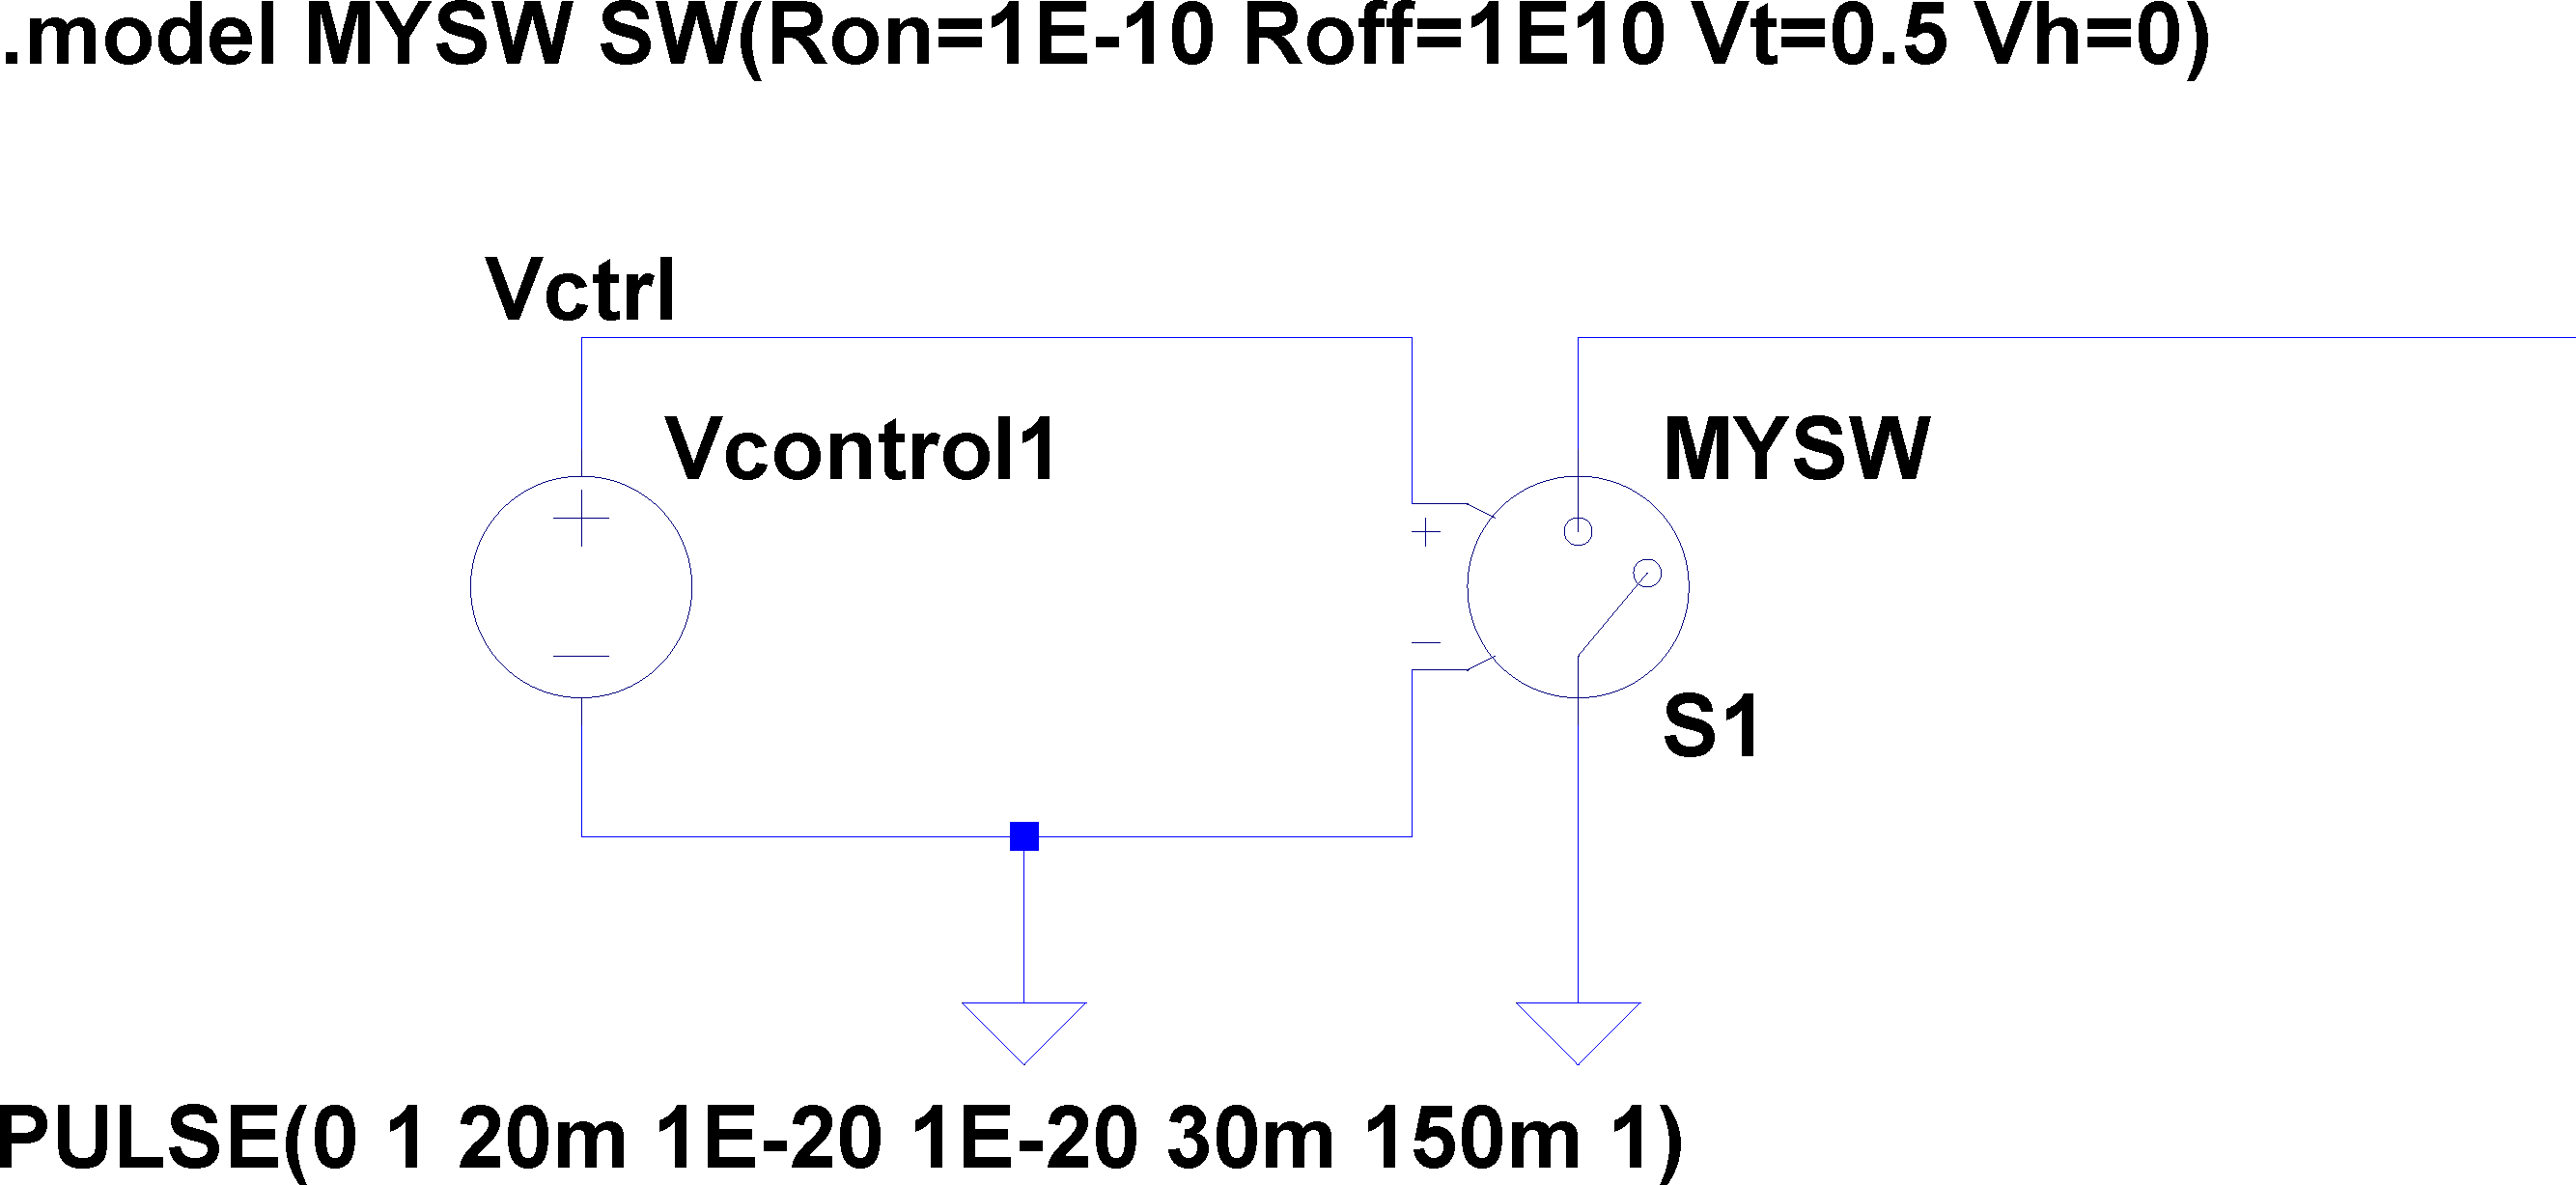
\includegraphics[width=0.9 \textwidth, angle=0]{./img/preguntas/p16a.png}
\caption{\label{fig:fig_p16_rl_switch}\footnotesize{Circuito usado para la conmutación de la carga}}
\end{center}
\end{figure}

%% Tensión de salida frente a saltos de carga de $0 A$ a $1 A$.


\textbf{INCOMPLETO}

\vfill

\clearpage
